% Adjusting chapter title format for regular (numbered) chapters
\titleformat{\chapter}[display]
  {\normalfont\huge\bfseries\centering}{\chaptertitlename\ \thechapter}{20pt}{\Huge}

% Using similar styling for unnumbered chapters but without "Chapter" prefix
\titleformat{name=\chapter,numberless}
  {\normalfont\huge\bfseries\centering}{}{0pt}{\Huge}

\titlespacing*{\chapter}{0pt}{50pt}{40pt} % Adjust vertical spacing before and after the title

\chapter{Introduction} % Ensures chapter numbering starts correctly
\label{chp:1}
\section{Background and Motivation}

Deep Neural Networks (DNNs) are increasingly being used in diverse applications due to their ability to match or exceed human-level performance. With the broader deployment of DNNs in various safety-critical systems like autonomous vehicles, healthcare, and avionics, concerns over their safety and trustworthiness have been raised \cite{ZhaoXBanks}. The availability of large datasets, fast computing methods, and their high performance has enabled the use of DNNs in safety-critical applications \cite{LeCun}. The critical nature of such applications makes it essential to thoroughly evaluate these DNNs before deployment to guarentee their reliability and safety.

\begin{figure}
  \centering
  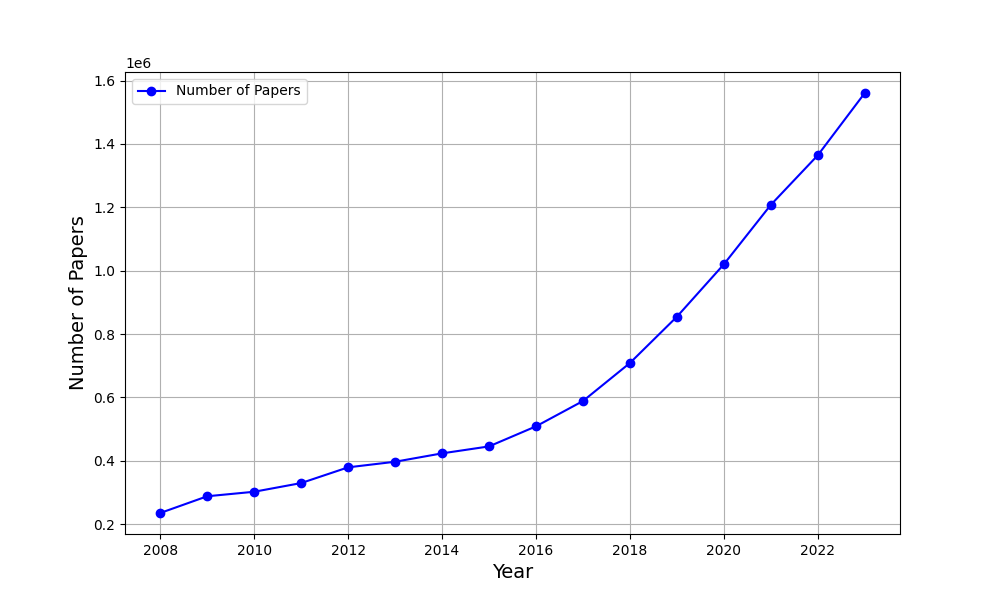
\includegraphics[width=0.65\textwidth]{Number of Published Papers on DNN Safety.png}
  \caption{Number of Published Papers on DNN Safety}
  \label{fig:publish}
\end{figure}

In recent years, there has been significant amount of publications focused on tackling this concern. Figure. \ref{fig:publish} visualizes the significant growth in the number of published papers related to DNNs safety from 2008 to 2023\footnote{The data is gathered using a comprehensive set of relevant keywords. The keywords used for data extraction include: 'deep neural network safety,' 'DNN verification,' 'DNN testing,' 'deep learning robustness,' 'neural network adversarial attacks,' 'DNN defense mechanisms,' 'DNN interpretability,' 'deep learning certification,' 'neural network validation,' and 'machine learning security.'}.


An important requirement for DNNs is that they are robust against input perturbations \cite{HuangX}. 
DNNs have shown a lack of robustness due to their vulnerability to adversarial examples, where even minor modifications to an input, sometimes imperceptible to humans, can destabilize the neural network \cite{Goodfellow,Carlini}. Unlike traditional software, DNNs do not have a clear control-flow structure. They learn their decision policy through training on large datasets, adjusting parameters gradually using various methods to achieve the desired accuracy. Figure. \ref{fig:Comparison} illustrates the flow of traditional software compared to neural network. Consequently, traditional software testing methods like functional coverage and branch coverage  cannot be applied to DNNs, thus challenging their use in safety-critical applications. This is because DNNs lack explicit paths and branches that can be directly tested; their behavior emerges from complex interactions within their learned parameters, making it difficult to apply traditional coverage metrics that rely on predefined control flows \cite{Sekhon}.

\begin{figure}
  \centering
  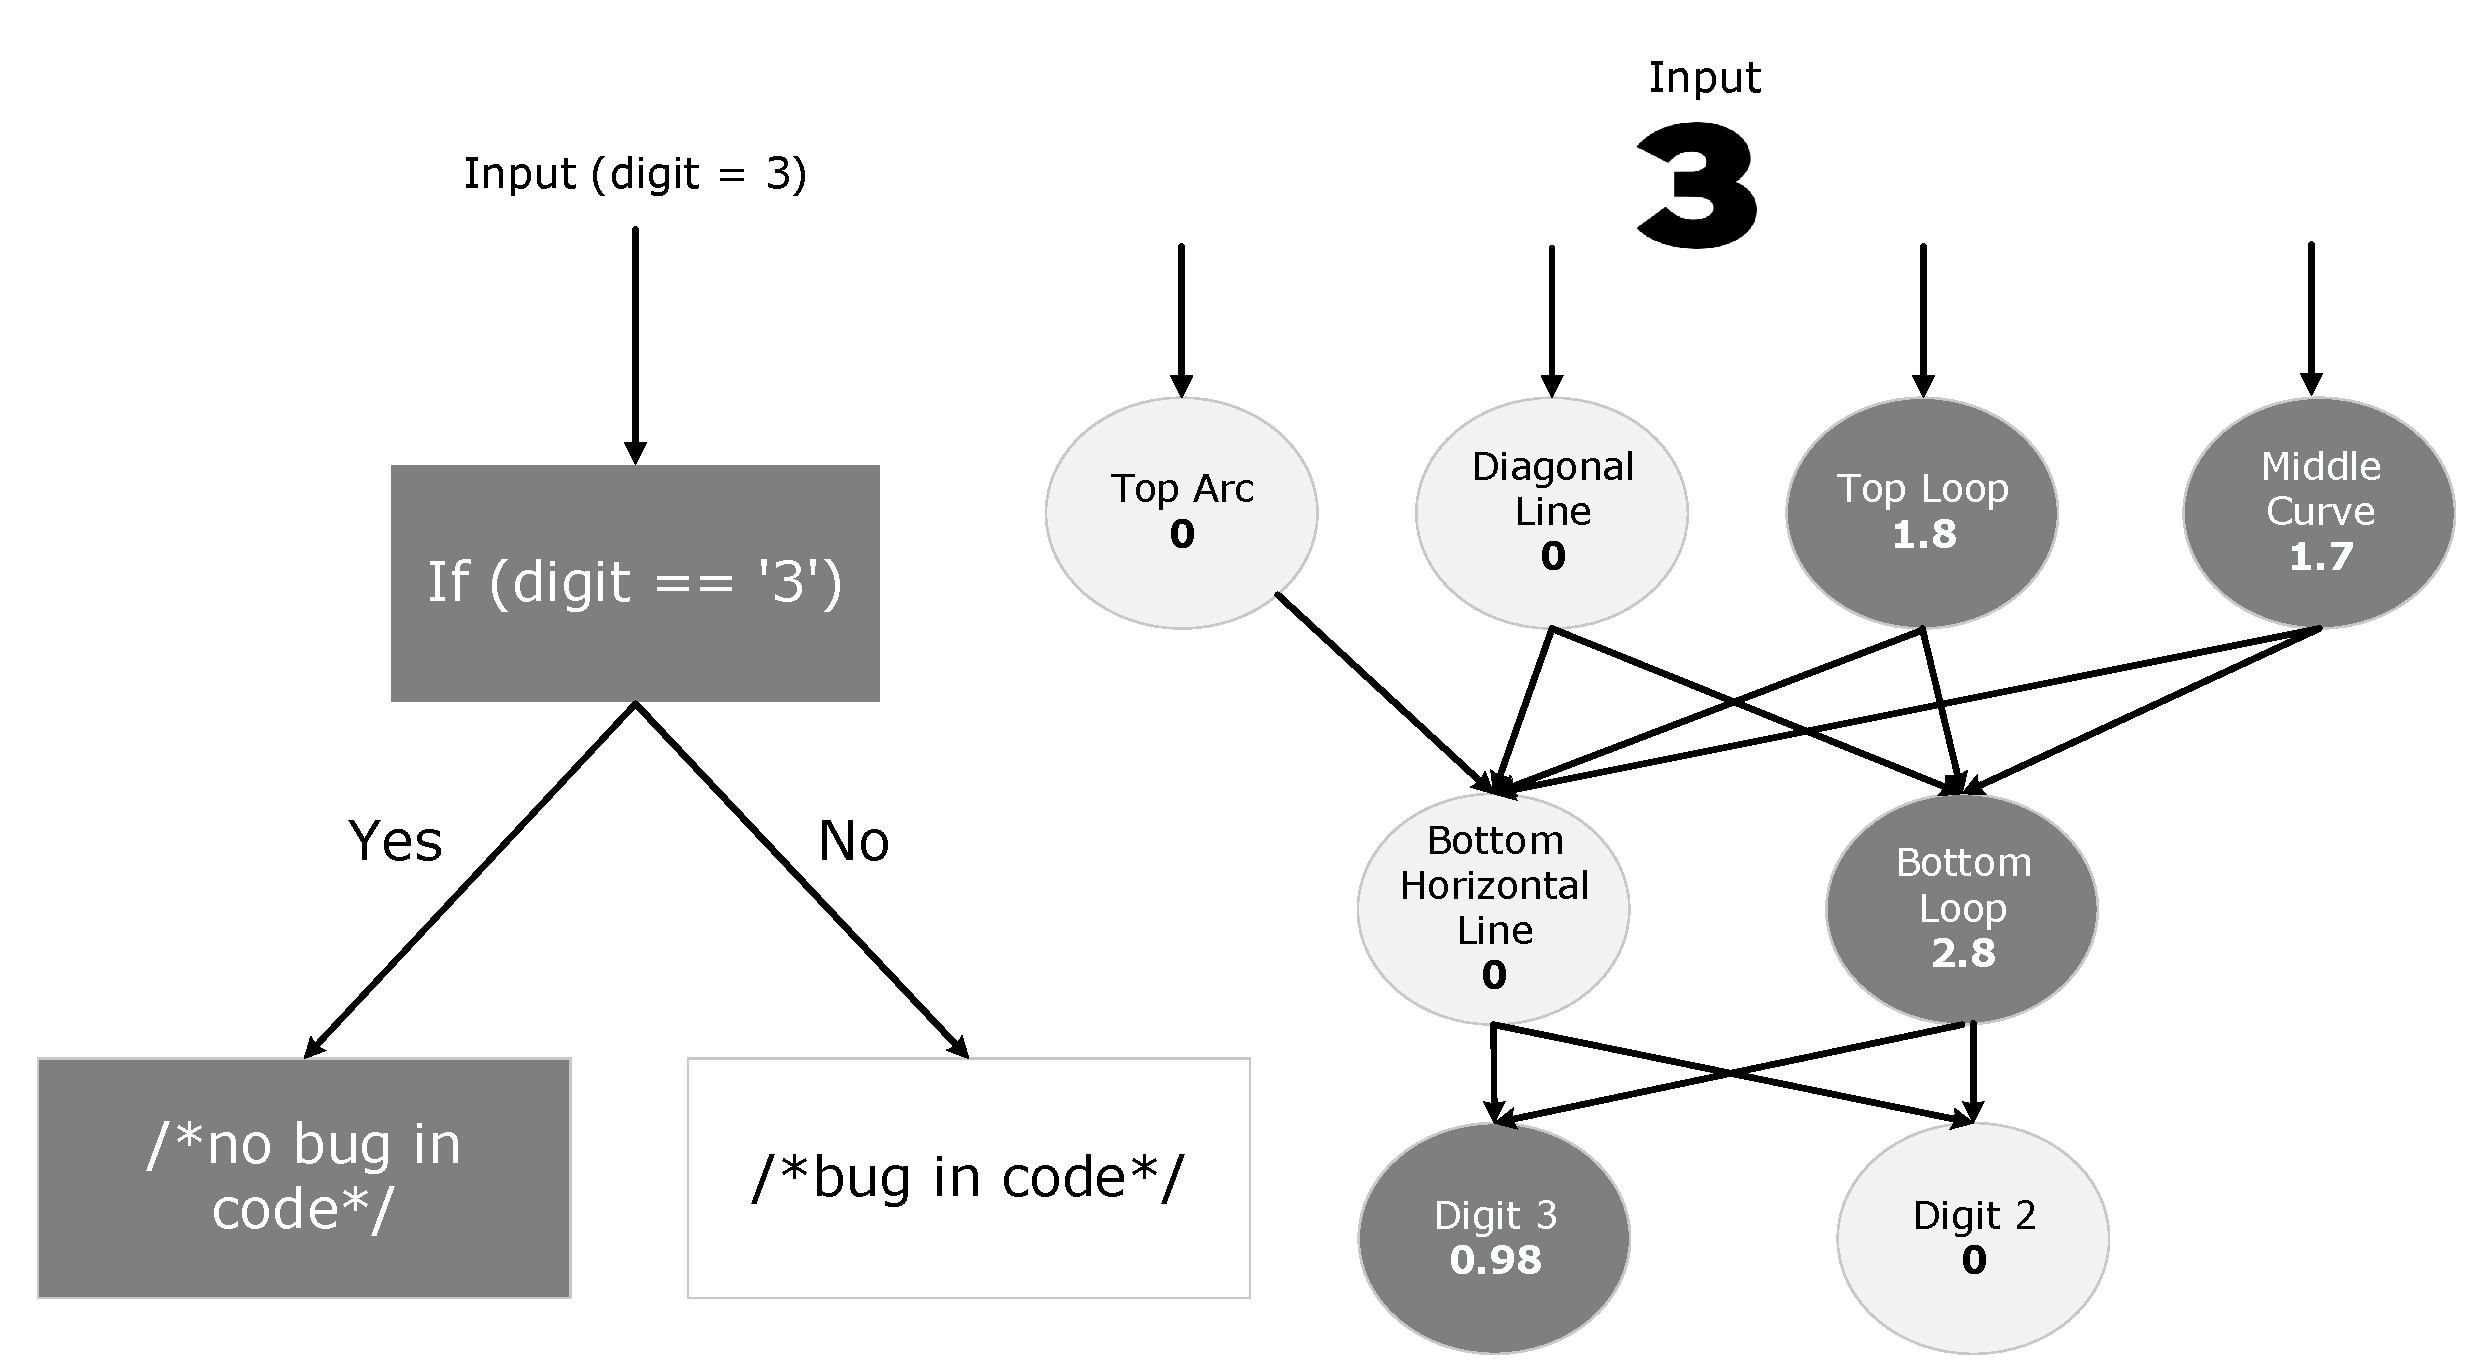
\includegraphics[width=0.75\textwidth]{traditionalandDNN.pdf}
  \caption{Comparison between program flows of a traditional program (left) and a neural network (right). The nodes in gray denote the corresponding basic blocks or neurons that participated while processing an input.}
  \label{fig:Comparison}
\end{figure}

In the past, researchers have extensively discussed both verification and testing techniques, which are useful for evaluating the DNNs. Verification involves proving the property (e.g. adversarial examples (noise, rotation, brightness, etc.)) of a system through mathematical proof. This approach ensures that certain property is met by the system based on a formal analysis. However,DNN verification techniques are promising, they suffer from a scalability problem, due to the high computational complexity and the large size of DNNs. Up to now, DNN verification techniques either work with small scale DNNs or with approximate methods with convergence guarantees on the bounds \cite{HuangX}. This limitation impacts the ability to achieve high coverage, which means to cover all input scenarios and conditions to ensure that all potential issues are identified.



On the other hand, testing focuses on identifying defects (i.e, counter example to a property) or provide assurance cases \cite{Rushby}, by evaluating the behavior of system through empirical methods. As a result, they can achieve high coverage, which suggests that more of a DNN's behavior has been tested and therefore the DNN has a lower chance of containing undetected bugs \cite{HuangX}. While these coverage metrics are useful, they often fall short in providing \hyperref[gloss]{\textsc{comprehensive}}\label{comprehensive} evaluations. This is because they primarily focus on the internal structure of the deep models, such as neuron activation patterns, rather than evaluating the DNNs behavior on a diverse set of inputs. This internal focus can miss identifying specific inputs that cause failures or unexpected behavior.


\begin{tcolorbox}[colback=purple!2!white, colframe=purple,title= 10\textsuperscript{th} Month Report Goal]

    The primary aim of my work in the first year is to review existing testing methods for assessing the robustness of DNNs, identify opportunities for improvement, and highlight the need for a fast, scalable, and generalizable end-to-end testing method. This report also aims to outline key research questions and objectives based on these findings and present initial contributions to the field.

\end{tcolorbox}
    

% \textcolor{olive}{ \textbf{Solution:} To address these limitations, I propose a complete framework that encompasses the entire process from specification to error summarization. This framework will introduce new coverage criteria driven by specific requirements and based on both local and global correctness. Local correctness involves evaluating the AI subsystem's performance on individual inputs representing specific classes, subjected to various transformations, ensuring that the model remains robust under specific conditions. Global correctness assesses the overall behavior of the AI system across a comprehensive range of scenarios, ensuring holistic robustness and reliability. By focusing on testing with specification-driven criteria, my approach aims to provide immediate feedback and uncover a wide range of issues, enhancing the robustness of DNNs.}


\section{Research Goal}

The primary goal of this research is to enhance the robustness of DNNs used in safety-critical systems by designing and implementing a comprehensive testing framework. This framework will formalize specifications related to model architecture, environmental properties and input data characteristics, including the type of data (e.g., images, text), size (e.g., number of samples), size for each class, and the number of classes involved.

The framework will adapt these specifications based on the \textbf{type of testing} being conducted. In \textbf{white-box testing}, full access to the model's internal details (e.g., number of neurons, layers, weights, and types of architectures like CNN, ResNet) is utilized to create precise adversarial examples using methods like FGSM. In \textbf{grey-box testing}, partial access allows the use of input-output pairs and basic model structures (e.g., general architecture without detailed parameters) to train surrogate models that approximate the target model's behavior, enabling the generation of effective test cases without need full internal details. In \textbf{black-box testing}, the framework relies on input-output behavior and environmental properties (e.g., expected input ranges, conditions like rain, dust, brightness, and noise) to iteratively probe and test the model's robustness without internal access. Defining these properties is crucial as it specifies the expected conditions the model should handle.

User requirements, such as specific modules to test and critical scenarios, as well as evaluation metrics (e.g., accuracy, precision, recall), will also be incorporated. If no specific requirements are provided, default parameters will ensure thorough assessment.However, it can also be customized for specific cases or multiple cases based on user specifications. For instance, a user might require the framework to focus on a particular class or scenario that is critical. This flexible and detailed approach aims to provide a robust method for testing DNNs in safety-critical environments.


To accurately identify weaknesses and areas for improvement, the framework will calculate both local coverage and global coverage using probabilistic programming language that allows you to define bayesian probability models and solve them automatically. This approach allows for a detailed analysis of the model's behavior under different conditions, providing insights into how the model performs in specific scenarios and overall. By examining local-level coverage, the framework can detect vulnerabilities that may arise in specific parts of the model or under particular conditions. Global-level coverage assessment, on the other hand, evaluates the model's overall stability across a wide range of scenarios. Together, these analyses help pinpoint specific vulnerabilities and highlight areas where the model can be improved, ultimately leading to more robust systems.

Additionally, the framework will generate a comprehensive error summary, providing insights into the types and frequencies of errors encountered. This summary will highlight critical failure points and suggest targeted improvements, enabling developers to enhance the system robustness.
Through continuous evaluation and iterative refinement, the framework aims to significantly enhance the safety and dependability of DNN models across different operational levels. This ongoing process ensures that the models remain robust and effective in a wide variety of real-world applications, ultimately contributing to their reliability in safety-critical systems.

\begin{tcolorbox}[colback=purple!2!white, colframe=purple,title= Thesis Goal]
   An end-to-end automated framework that thoroughly integrates data, test cases, and test coverage according to given specifications and provides a detailed error summary.
\end{tcolorbox}

\section{Research Questions and Objectives}
\label{Research Questions and Objectives}
This section outlines the research questions and their corresponding objectives.


\begin{enumerate}

    \item \textbf{How can we design a comprehensive framework to test system robustness?} Create a framework that test the DNN under a variety of conditions, ensuring it meets performance standards even in edge cases and adverse scenarios \textbf{(Obj1)}.

  
    \item \textbf{How can we clearly define and specify the properties of the system?} Formalize specifications by developing templates and a specification language that enable users to clearly define and specify the properties of the system and its associated data for testing purposes \textbf{(Obj2)}.

    
    \item \textbf{How can we sample inputs efficiently?}Develop a sampling approach that effectively identifies and prioritizes corner cases. It can be used to guide best selection of inputs for test case generation\textbf{(Obj3)}.
    
    \item \textbf{Can interpretability analysis aid in effective test case generation?} Implement interpretability analysis to identify and prioritize key influential features in the DNN testing process, exploring the use of high influential features for effective test case generation\textbf{(Obj4)}.
   
    \item \textbf{How can we generate highly effective test cases that ensure complete coverage?} Generate highly effective test cases by first developing a sampling approach to collect efficient samples, and then using these samples to identify critical pixels. The identified critical pixels will form the basis for creating test cases that ensure complete coverage and thoroughly assess model vulnerabilities\textbf{(Obj5)}.
 
    \item \textbf{How can we ensure comprehensive test coverage for deep learning models?} Integrate advanced probabilistic methods to evaluate both \hyperref[gloss]{\textsc{\textsc{local coverage}}} \label{Local coverage} and \hyperref[gloss]{\textsc{\textsc{global coverage}}} \label{Global coverage} \textbf{(Obj6)}.
               
    \item \textbf{How can error summarization be employed to quantify the impacts on model robustness?} Develop method for error summarization that analyze the results of DNNs testing to identify weaknesses. This method will help quantify the impacts of errors on model robustness and provide insights into areas requiring improvement\textbf{(Obj7)}.
  

  
\end{enumerate}




\section{Contribution of this Report}

This research makes the following key contributions to the field of deep learning correctness evaluation:

\begin{itemize}
    \item An \textit{\textcolor{blue}{end-to-end pipeline}} is designed for evaluating the robustness of the system Chapter \ref{chp:3}.
    \item A \textit{\textcolor{blue}{hybrid sampling}} technique is proposed to identify and prioritize the corner cases Chapter \ref{chp:3}.
    \item A \textit{\textcolor{blue}{conceptual framework}} is proposed that quantifies both local and global robustness. This framework uses Problog, a probabilistic logic programming language, to verify system global robustness Chapter \ref{chp:3}. 
    \item An \textit{\textcolor{blue}{interpretability-driven test case generation}} approach is employed to pinpoint critical input features, which are then used to create test cases with a higher probability of inducing mispredictions, thus effectively evaluating and enhancing model robustness Chapter \ref{chp:3}.
    % \item A novel \textit{error summarization} approach is introduced, which helps in better identifying where model makes mistakes, especially in relation to specific classes and property.
    \item All \textit{\textcolor{blue}{experiments}} are conducted using publicly available datasets, including DAWN, CIFAR, and MNIST Chapter \ref{chp:3}.
\end{itemize}

\begin{center}
    \fcolorbox{gray}{lightgray}{
    \parbox{0.95\linewidth}{
    \textbf{Note:} The contributions of this report do not include methods for defining system properties and error summarization technique. Additionally, adversarial examples used in the experiments are taken from existing literature.
    }
    }
    \end{center}
\section{Organization of the Thesis}\hypertarget{organization of thesis}{}
The remainder of the thesis is organized as follows: related studies are presented in Chapter \ref{chp:2}. The system model and proposed methodology are demonstrated in Chapter \ref{chp:3}. Chapter \ref{chp:4} describes the simulation results of our proposed schemes. Finally, the the next two year Phd plan is presented in Chapter \ref{chp:9}.


\clearpage
